% begin module cylindrical-shells-intro
\begin{frame}
Find the volume of the solid obtained by rotating the region bounded by $y = 2x^2 - x^3$ and the $x$-axis around $\ldots$
\begin{tabular}{p{6cm}@{\ }p{6cm}}
\ \only<handout:0| -1>{%
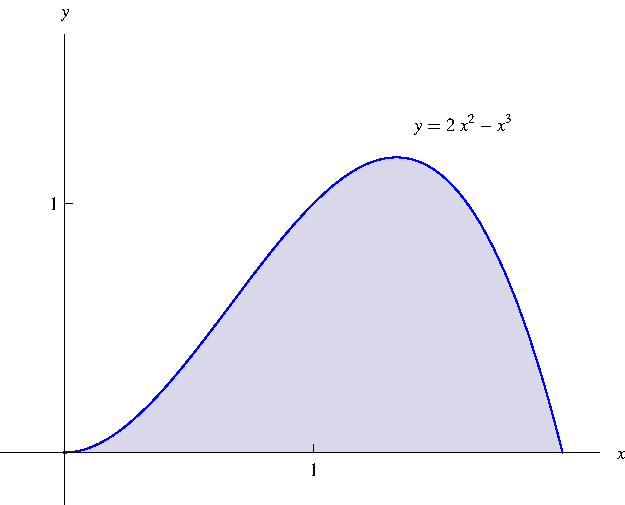
\includegraphics[height=4cm]{volumes/pictures/06-03-setupz.pdf}%
}%
\only<2->{%
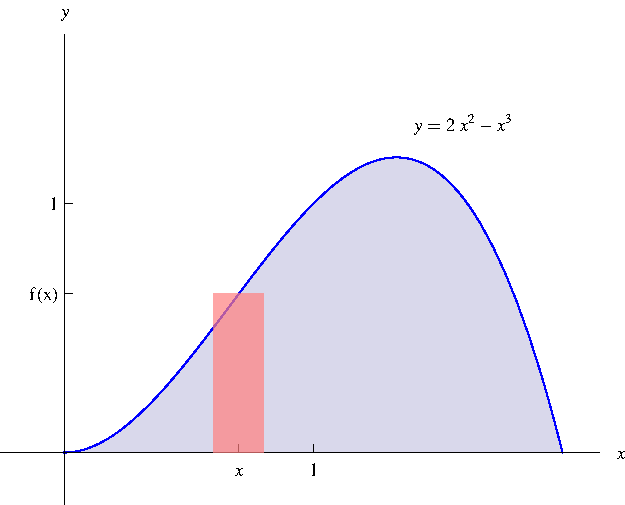
\includegraphics[height=4cm]{volumes/pictures/06-03-setupa.pdf}%
}%
&%
\ \only<handout:0| -4>{%
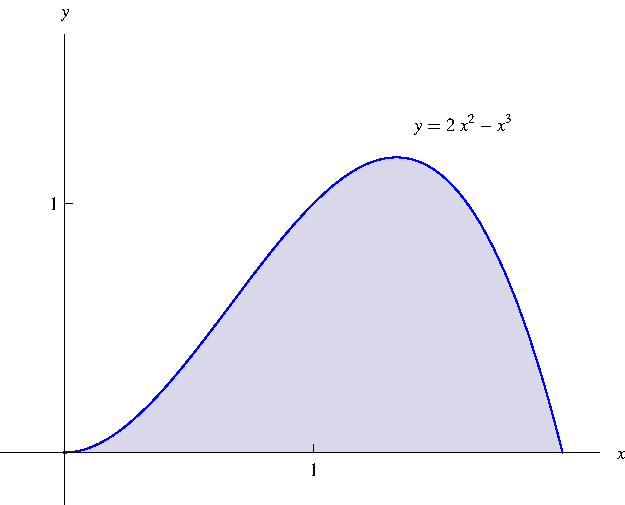
\includegraphics[height=4cm]{volumes/pictures/06-03-setupz.pdf}%
}%
\only<5->{%
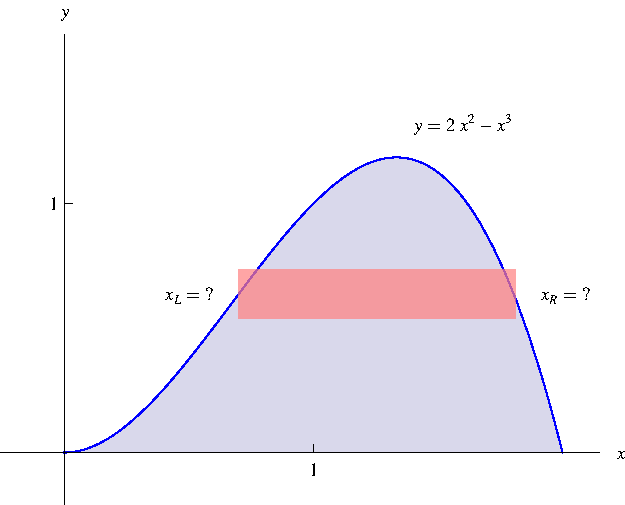
\includegraphics[height=4cm]{volumes/pictures/06-03-setupb.pdf}%
}%
\\%
\begin{itemize}
\item<1->  $\ldots$ the $x$-axis.
\item<2->  Approximate the volume using circular cylinders with radius $2x^2 - x^3$ and height $\Delta x$.
\item<3->  $V = \int_0^2 \pi (2x^2 - x^3)^2 \diff x$.
\item<4->  We can solve this.
\end{itemize}
&%
\begin{itemize}
\item<1->  $\ldots$ the $y$-axis.
\item<5->  Approximate the volume using circular cylinders with radii $x_R$ and $x_L$.
\item<6->  We don't know $x_R$ and $x_L$.
\item<7->  We need new techniques.
\end{itemize}
\end{tabular}
\end{frame}
% end module cylindrical-shells-intro
